\documentclass{beamer}
\usepackage[utf8]{inputenc}

\usetheme{Madrid}
\usecolortheme{default}
\usepackage{amsmath,amssymb,amsfonts,amsthm}
\usepackage{txfonts}
\usepackage{tikz}
\usepackage{graphicx}
\usepackage{listings}
\usepackage{adjustbox}
\usepackage{array}
\usepackage{tabularx}
\usepackage{gvv}
\usepackage{lmodern}
\usepackage{circuitikz}

\setbeamertemplate{page number in head/foot}[totalframenumber]

\usepackage{tcolorbox}
\tcbuselibrary{minted,breakable,xparse,skins}

\definecolor{bg}{gray}{0.95}
\DeclareTCBListing{mintedbox}{O{}m!O{}}{%
  breakable=true,
  listing engine=minted,
  listing only,
  minted language=#2,
  minted style=default,
  minted options={%
    linenos,
    gobble=0,
    breaklines=true,
    breakafter=,,
    fontsize=\small,
    numbersep=8pt,
    #1},
  boxsep=0pt,
  left skip=0pt,
  right skip=0pt,
  left=25pt,
  right=0pt,
  top=3pt,
  bottom=3pt,
  arc=5pt,
  leftrule=0pt,
  rightrule=0pt,
  bottomrule=2pt,
  toprule=2pt,
  colback=bg,
  colframe=orange!70,
  enhanced,
  overlay={%
    \begin{tcbclipinterior}
    \fill[orange!20!white] (frame.south west) rectangle ([xshift=20pt]frame.north west);
    \end{tcbclipinterior}},
  #3,
}

\lstset{
    language=C,
    basicstyle=\ttfamily\small,
    keywordstyle=\color{blue},
    stringstyle=\color{orange},
    commentstyle=\color{green!60!black},
    numbers=left,
    numberstyle=\tiny\color{gray},
    breaklines=true,
    showstringspaces=false,
}

%------------------------------------------------------------
\title{2.3.12}
\date{3rd September 2025}
\author{Anshu kumar ram - EE25BTECH11009}

\begin{document}

\frame{\titlepage}

% ---------------- Question ----------------
\begin{frame}{Question}
Find the angle which the line
\[
\frac{x}{1} = \frac{y}{-1} = \frac{z}{0}
\]
makes with the positive direction of the Y-axis.
\end{frame}

% ---------------- Solution Step 1 ----------------
\begin{frame}{Solution Step 1}
The line can be written as
\[
L : \vec{x} = \myvec{0\\0\\0} + k\myvec{1\\-1\\0}
\]

So, the direction vector is
\[
\vec{v} = \myvec{1\\-1\\0}, \quad 
\vec{e_2} = \myvec{0\\1\\0}
\]
\end{frame}

% ---------------- Solution Step 2 ----------------
\begin{frame}{Solution Step 2}
Compute dot product:
\begin{align}
\vec{v}^T \vec{e_2} &= \myvec{1 & -1 & 0}\myvec{0\\1\\0} = -1
\end{align}

Norms:
\begin{align}
\|\vec{v}\| &= \sqrt{1^2 + (-1)^2 + 0^2} = \sqrt{2} \\
\|\vec{e_2}\| &= 1
\end{align}
\end{frame}

% ---------------- Solution Step 3 ----------------
\begin{frame}{Solution Step 3}
Angle:
\begin{align}
\cos \theta &= \frac{\vec{v}^T\vec{e_2}}{\|\vec{v}\|\|\vec{e_2}\|} 
= \frac{-1}{\sqrt{2}} \\
\theta &= \cos^{-1}\!\left(-\tfrac{1}{\sqrt{2}}\right)
= 135^\circ
\end{align}

\[
\boxed{\theta = 135^\circ}
\]
\end{frame}
% ---------------- Plot ----------------
\begin{frame}{Plot}
\centering
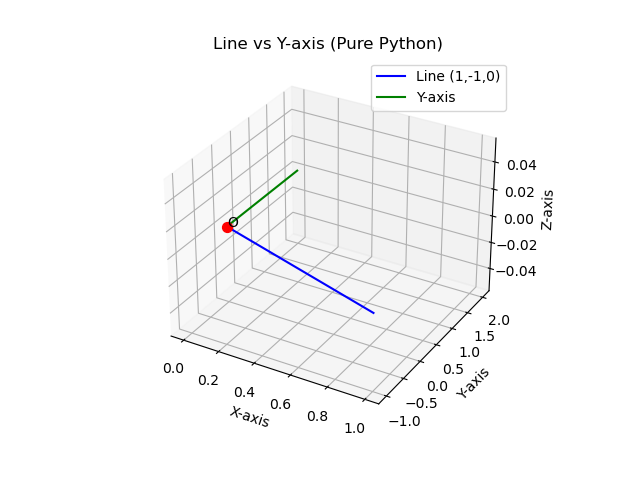
\includegraphics[width=\columnwidth, height=0.8\textheight, keepaspectratio]{figs/line.png}
\end{frame}

% ---------------- C Code ----------------
\begin{frame}[fragile]{C Code (angle\_between)}
\begin{lstlisting}[language=C]
#include <stdio.h>
#include <math.h>

// Function to compute angle between two 3D vectors
double angle_between(double *u, double *v) {
    double dot = u[0]*v[0] + u[1]*v[1] + u[2]*v[2];
    double norm_u = sqrt(u[0]*u[0] + u[1]*u[1] + u[2]*u[2]);
    double norm_v = sqrt(v[0]*v[0] + v[1]*v[1] + v[2]*v[2]);
    double cos_theta = dot / (norm_u * norm_v);
    if(cos_theta > 1.0) cos_theta = 1.0;
    if(cos_theta < -1.0) cos_theta = -1.0;
    return acos(cos_theta);
}
\end{lstlisting}
\end{frame}

% ---------------- Python + C ----------------
\begin{frame}[fragile]{Python + C (Part 1)}
\begin{lstlisting}[language=Python]
import ctypes
import numpy as np
import matplotlib.pyplot as plt

handc = ctypes.CDLL("./func.so")
handc.angle_between.argtypes = [
    ctypes.POINTER(ctypes.c_double),
    ctypes.POINTER(ctypes.c_double)
]
handc.angle_between.restype = ctypes.c_double

def np_to_c(arr):
    return arr.ctypes.data_as(ctypes.POINTER(ctypes.c_double))

v = np.array([1.0,-1.0,0.0], dtype=np.float64)
e2 = np.array([0.0,1.0,0.0], dtype=np.float64)

theta = handc.angle_between(np_to_c(v), np_to_c(e2))
theta_deg = np.degrees(theta)
print(f"Angle = {theta_deg:.2f} degrees")
\end{lstlisting}
\end{frame}

\begin{frame}[fragile]{Python + C (Part 2)}
\begin{lstlisting}[language=Python]
fig = plt.figure()
ax = fig.add_subplot(111, projection='3d')

t = np.linspace(-2,2,10)
x_line, y_line, z_line = t*v[0], t*v[1], t*v[2]
ax.plot(x_line, y_line, z_line, label='Line (1,-1,0)')

ax.plot([0,0],[0,2],[0,0],'g',label='Y-axis')

ax.set_xlabel('X'); ax.set_ylabel('Y'); ax.set_zlabel('Z')
ax.legend()
ax.set_title(f"Angle ≈ {theta_deg:.1f}°")
plt.savefig("../figs/line_c.png")
plt.show()
\end{lstlisting}
\end{frame}

% ---------------- Pure Python ----------------
\begin{frame}[fragile]{Pure Python (Part 1)}
\begin{lstlisting}[language=Python]
import sys
sys.path.insert(0, '/home/anshu-ram/matgeo/codes/CoordGeo')

import numpy as np
import matplotlib.pyplot as plt
from line.funcs import line_gen

v = np.array([1,-1,0]).reshape(-1,1)
e2 = np.array([0,1,0]).reshape(-1,1)

dot = float(v.T @ e2)
theta_rad = np.arccos(dot/(np.linalg.norm(v)*np.linalg.norm(e2)))
theta_deg = np.degrees(theta_rad)
print(f"Angle = {theta_deg:.2f} degrees")
\end{lstlisting}
\end{frame}

\begin{frame}[fragile]{Pure Python (Part 2)}
\begin{lstlisting}[language=Python]
A = np.zeros((3,1))
B = v
line_points = line_gen(A, B)

Y_end = np.array([0,2,0]).reshape(-1,1)
yaxis_points = line_gen(A, Y_end)

fig = plt.figure()
ax = fig.add_subplot(111, projection='3d')
ax.plot(line_points[0,:], line_points[1,:], line_points[2,:], label="Line")
ax.plot(yaxis_points[0,:], yaxis_points[1,:], yaxis_points[2,:], label="Y-axis")

ax.scatter(0,0,0,color="red",s=50)
ax.text(0,0,0,"O",fontsize=10)
ax.set_xlabel("X"); ax.set_ylabel("Y"); ax.set_zlabel("Z")
ax.legend(); plt.title("Line vs Y-axis")
plt.savefig("../figs/line.png"); plt.show()
\end{lstlisting}
\end{frame}



\end{document}
